% Options for packages loaded elsewhere
\PassOptionsToPackage{unicode}{hyperref}
\PassOptionsToPackage{hyphens}{url}
%
\documentclass[
]{article}
\usepackage{amsmath,amssymb}
\usepackage{iftex}
\ifPDFTeX
  \usepackage[T1]{fontenc}
  \usepackage[utf8]{inputenc}
  \usepackage{textcomp} % provide euro and other symbols
\else % if luatex or xetex
  \usepackage{unicode-math} % this also loads fontspec
  \defaultfontfeatures{Scale=MatchLowercase}
  \defaultfontfeatures[\rmfamily]{Ligatures=TeX,Scale=1}
\fi
\usepackage{lmodern}
\ifPDFTeX\else
  % xetex/luatex font selection
\fi
% Use upquote if available, for straight quotes in verbatim environments
\IfFileExists{upquote.sty}{\usepackage{upquote}}{}
\IfFileExists{microtype.sty}{% use microtype if available
  \usepackage[]{microtype}
  \UseMicrotypeSet[protrusion]{basicmath} % disable protrusion for tt fonts
}{}
\makeatletter
\@ifundefined{KOMAClassName}{% if non-KOMA class
  \IfFileExists{parskip.sty}{%
    \usepackage{parskip}
  }{% else
    \setlength{\parindent}{0pt}
    \setlength{\parskip}{6pt plus 2pt minus 1pt}}
}{% if KOMA class
  \KOMAoptions{parskip=half}}
\makeatother
\usepackage{xcolor}
\usepackage[margin=1in]{geometry}
\usepackage{color}
\usepackage{fancyvrb}
\newcommand{\VerbBar}{|}
\newcommand{\VERB}{\Verb[commandchars=\\\{\}]}
\DefineVerbatimEnvironment{Highlighting}{Verbatim}{commandchars=\\\{\}}
% Add ',fontsize=\small' for more characters per line
\usepackage{framed}
\definecolor{shadecolor}{RGB}{248,248,248}
\newenvironment{Shaded}{\begin{snugshade}}{\end{snugshade}}
\newcommand{\AlertTok}[1]{\textcolor[rgb]{0.94,0.16,0.16}{#1}}
\newcommand{\AnnotationTok}[1]{\textcolor[rgb]{0.56,0.35,0.01}{\textbf{\textit{#1}}}}
\newcommand{\AttributeTok}[1]{\textcolor[rgb]{0.13,0.29,0.53}{#1}}
\newcommand{\BaseNTok}[1]{\textcolor[rgb]{0.00,0.00,0.81}{#1}}
\newcommand{\BuiltInTok}[1]{#1}
\newcommand{\CharTok}[1]{\textcolor[rgb]{0.31,0.60,0.02}{#1}}
\newcommand{\CommentTok}[1]{\textcolor[rgb]{0.56,0.35,0.01}{\textit{#1}}}
\newcommand{\CommentVarTok}[1]{\textcolor[rgb]{0.56,0.35,0.01}{\textbf{\textit{#1}}}}
\newcommand{\ConstantTok}[1]{\textcolor[rgb]{0.56,0.35,0.01}{#1}}
\newcommand{\ControlFlowTok}[1]{\textcolor[rgb]{0.13,0.29,0.53}{\textbf{#1}}}
\newcommand{\DataTypeTok}[1]{\textcolor[rgb]{0.13,0.29,0.53}{#1}}
\newcommand{\DecValTok}[1]{\textcolor[rgb]{0.00,0.00,0.81}{#1}}
\newcommand{\DocumentationTok}[1]{\textcolor[rgb]{0.56,0.35,0.01}{\textbf{\textit{#1}}}}
\newcommand{\ErrorTok}[1]{\textcolor[rgb]{0.64,0.00,0.00}{\textbf{#1}}}
\newcommand{\ExtensionTok}[1]{#1}
\newcommand{\FloatTok}[1]{\textcolor[rgb]{0.00,0.00,0.81}{#1}}
\newcommand{\FunctionTok}[1]{\textcolor[rgb]{0.13,0.29,0.53}{\textbf{#1}}}
\newcommand{\ImportTok}[1]{#1}
\newcommand{\InformationTok}[1]{\textcolor[rgb]{0.56,0.35,0.01}{\textbf{\textit{#1}}}}
\newcommand{\KeywordTok}[1]{\textcolor[rgb]{0.13,0.29,0.53}{\textbf{#1}}}
\newcommand{\NormalTok}[1]{#1}
\newcommand{\OperatorTok}[1]{\textcolor[rgb]{0.81,0.36,0.00}{\textbf{#1}}}
\newcommand{\OtherTok}[1]{\textcolor[rgb]{0.56,0.35,0.01}{#1}}
\newcommand{\PreprocessorTok}[1]{\textcolor[rgb]{0.56,0.35,0.01}{\textit{#1}}}
\newcommand{\RegionMarkerTok}[1]{#1}
\newcommand{\SpecialCharTok}[1]{\textcolor[rgb]{0.81,0.36,0.00}{\textbf{#1}}}
\newcommand{\SpecialStringTok}[1]{\textcolor[rgb]{0.31,0.60,0.02}{#1}}
\newcommand{\StringTok}[1]{\textcolor[rgb]{0.31,0.60,0.02}{#1}}
\newcommand{\VariableTok}[1]{\textcolor[rgb]{0.00,0.00,0.00}{#1}}
\newcommand{\VerbatimStringTok}[1]{\textcolor[rgb]{0.31,0.60,0.02}{#1}}
\newcommand{\WarningTok}[1]{\textcolor[rgb]{0.56,0.35,0.01}{\textbf{\textit{#1}}}}
\usepackage{graphicx}
\makeatletter
\def\maxwidth{\ifdim\Gin@nat@width>\linewidth\linewidth\else\Gin@nat@width\fi}
\def\maxheight{\ifdim\Gin@nat@height>\textheight\textheight\else\Gin@nat@height\fi}
\makeatother
% Scale images if necessary, so that they will not overflow the page
% margins by default, and it is still possible to overwrite the defaults
% using explicit options in \includegraphics[width, height, ...]{}
\setkeys{Gin}{width=\maxwidth,height=\maxheight,keepaspectratio}
% Set default figure placement to htbp
\makeatletter
\def\fps@figure{htbp}
\makeatother
\setlength{\emergencystretch}{3em} % prevent overfull lines
\providecommand{\tightlist}{%
  \setlength{\itemsep}{0pt}\setlength{\parskip}{0pt}}
\setcounter{secnumdepth}{-\maxdimen} % remove section numbering
\usepackage{titling}
\usepackage{mdframed}
\usepackage{cancel}
\usepackage{amsmath}
\usepackage{sectsty}
\pretitle{\begin{center}\Huge\bfseries}
\posttitle{\end{center}\vspace{0.7cm}}
\preauthor{\begin{center}\Large}
\postauthor{\end{center}\vspace{0.3cm}}
\predate{\begin{center}\large}
\postdate{\end{center}\vspace{0.3cm}}
\ifLuaTeX
  \usepackage{selnolig}  % disable illegal ligatures
\fi
\IfFileExists{bookmark.sty}{\usepackage{bookmark}}{\usepackage{hyperref}}
\IfFileExists{xurl.sty}{\usepackage{xurl}}{} % add URL line breaks if available
\urlstyle{same}
\hypersetup{
  pdfkeywords={distribución muestral, variables aleatorias discretas,
simulación en R-Software, histogramas},
  hidelinks,
  pdfcreator={LaTeX via pandoc}}

\author{}
\date{\vspace{-2.5em}}

\begin{document}

\begin{titlepage}
  \title{Simulación de un dado justo lanzado \\ 3 veces consecutivas. \\ Estudio de variables aleatorias discretas.}
  \author{Angel Granados \\ {\small @aggranadoss}}
  \maketitle
  \begin{abstract}
    El presente estudio se centra en la distribución de la media muestral de los resultados obtenidos al lanzar un dado no cargado tres veces. Se plantea determinar la media y la desviación estándar y encontrar la distribución de la muestra. Las simulaciones se harán en R-Software examinando e identificando la repetición de ciertos valores y su distribución tanto de forma teórica como observando en el histograma resultante de los valores simulados.
    
    \textbf{Palabras clave:} distribución muestral, variables aleatorias discretas, simulación en R-Software, histogramas
  \end{abstract}
\end{titlepage}

\hypertarget{introducciuxf3n}{%
\section{1. Introducción}\label{introducciuxf3n}}

Consideraremos el lanzamiento de un dado justo (sin cargar) de tal forma que se lanzará 3 veces consecutivas en una muestra que consideraremos "grande" Toda la teoría se sustentará en el libro de Inferencia Estadística del Wackerly-Mendenhall-Scheaffer. Se responderán a las preguntas ¿Cuáles son la media $\mu_{\bar{Y}}$  y la desviación estándar $\sigma_{\bar{Y}}$ , de $\bar{Y}$ ? ¿Cómo podemos determinar la
distribución muestral de $\bar{Y}$? justificadas desde la teoría. El ejercicio se encuentra en el libro de Inferencia Estadística, solo que aca se justificará el detalle de las cuentas y la construcción del modelo hasta su solución. Se trabajará en una simulación para representar y comparar con el resultado teórico.     

\hypertarget{soporte-teuxf3rico}{%
\section{2. Soporte Teórico}\label{soporte-teuxf3rico}}

\definecolor{lightgray}{RGB}{240,240,240}
\newenvironment{cajainferencia}{
  \begin{center}
  \begin{minipage}{0.9\textwidth}
  \begin{mdframed}[backgroundcolor=lightgray,linewidth=0pt]
}{
  \end{mdframed}
  \end{minipage}
  \end{center}
}


Para el estudio del dado, la variable aleatoria que tomaremos será discreta ya que puede tomar sólo un número finito de valores distintos y la probabilidad de que $P(\bar{Y}=y_i)$ tome el valor de $y_i$ se definirá como la suma de las probabilidades de todos los puntos muestrales a los que se le asigna el valor de $y_i$. 

La distribución de probabilidad para una variable discreta la representaremos como un histograma y para cualquier distribución de probabilidad discreta, debe cumplirse que:

\begin{itemize}
  
  \item $0 \leq p(y) \leq 1$ para todo $y$
  
  \item $\displaystyle \sum_{y} p(y)=1$
\end{itemize}

Usaremos los siguientes teoremas, definiciones y ejemplos del texto de Inferencia Estadística del Wackerly:

\begin{cajainferencia}
\textbf{Teorema 3.2}

Sea $Y$ una variable aleatoria discreta con función de probabilidad $p(y)$ y sea $g(Y)$ una función de valor real de $Y$. Entonces, el valor esperado de $g(Y)$ está dado por: 

$$ E[g(Y)] = g(y)p(y)$$

\end{cajainferencia}



\begin{cajainferencia}
\textbf{Varianza y desviación estándar}

Sea $Y$ una variable aleatoria con media $E(Y)=\mu$, la varianza de una variable aleatoria $Y$ se define como el valor esperado de $(Y-\mu)^{2}$. Esto es,

$$ V(Y) = E[(Y-\mu)^{2}]$$

\end{cajainferencia}


\begin{cajainferencia}

  \textbf{Teorema 5.12}
    
    Sean $Y_{1},Y_{2},\cdots, Y_{n}$ y $X_{1},X_{2},\cdots, X_{m}$ variables aleatorias con $E(Y_{i})=\mu_{i}$ y $E(X_{j})=\alpha_{j}$
se define

$$U_{1} = \sum_{i=1}^{n}a_{i}Y_{i} \hspace{0.5cm} \text{ y } \hspace{0.5cm} U_{2} = \sum_{j=1}^{m}b_{j}X_{j} $$

con constantes $a_{i} \text{ y } b_{j}$. Entonces se cumple lo siguiente:

\vspace{0.2cm}

\begin{enumerate}
    
    \item $E[U_{1}] = \sum_{i=1}^{n}a_{i}\mu_{i}$
    
    \item $ \displaystyle V(U_{1}) = \sum_{i=1}^{n}a_{i}^{2}V(Y_{i}) + 2\sum \sum_{1\leq i \leq j \leq n} a_{i}a_{j} Cov(Y_{i},Y_{j}) $.
    
    \item $\displaystyle Cov(U_{1},U_{2}) = \sum_{i=1}^{n} \sum_{j=1}^{m} a_{i}b_{j} Cov(Y_{i},X_{j}) $
  
\end{enumerate}
  

\end{cajainferencia}

\begin{cajainferencia}

\textbf{Ejemplo 5.27}

Sean $Y_{1},Y_{2}, \cdots ,Y_{n}$ variables aleatorias independientes con $E(Y_{i}) = \mu$ y $V(Y_{i}) = \sigma^{2}$. (Estas
variables pueden denotar los resultados de n intentos independientes de un experimento.) Se define

$$\bar{Y}= \frac{1}{n}\sum_{i=1}{n}Y_{i}$$

se demuestra que $\displaystyle E(\bar{Y})=\mu \text{ y } V(\bar{Y}) = \frac{\sigma^2}{n}$

\end{cajainferencia}


\hypertarget{ejemplo-ilustrativo}{%
\section{3. Ejemplo Ilustrativo}\label{ejemplo-ilustrativo}}

Un dado sin estar cargado se lanza tres veces. Sean $Y_{1}$, $Y_{2}$ y $Y_{3}$ el número de puntos vistos en la cara superior para los tiros $1$, $2$ y $3$, respectivamente. Suponga que estamos interesados en $\bar{Y} = (Y_{1} + Y_{2} + Y_{3} )/3$, el número promedio de puntos vistos en una muestra de tamaño $3$. ¿Cuáles son la media $\mu_{\bar{y}}$  y la desviación estándar $\sigma_{\bar{y}}$ , de $\bar{Y}$ ? ¿Cómo podemos determinar la
distribución muestral de $\bar{Y}$ ?


\textbf{Solución del ejercicio:}

\definecolor{lightgray}{RGB}{240,240,240}
\newenvironment{caja}{
  \begin{center}
  \begin{minipage}{0.9\textwidth}
  \begin{mdframed}[backgroundcolor=lightgray,linewidth=0pt]
}{
  \end{mdframed}
  \end{minipage}
  \end{center}
}


Como el dado no está cargado, la probabilidad de que caiga un número arbitrario del conjunto $y_{i} \in \{1,\cdots,6\}$ es $p(y_{i}) = \displaystyle \frac{1}{6}$ con $i \in \{1,\cdots,6\}$ definido de la forma $y_{i} = i$. Respondiendo a la pregunta  ¿Cuál es la media 
$\mu_{\bar{y}}$? se tiene que el cálculo de la media está dado: 

$$\mu = \frac{1}{n} \sum_{i=1}^{n}y_{i} \hspace{1.5cm} (3.1)$$

por (3.1) se tiene:

\begin{itemize}
  \item $\displaystyle \mu = \frac{1}{6}\sum_{i=1}^{6}y_{i}$
  
  $\displaystyle \hspace{0.4cm} = \frac{1}{6} [1+\cdots +6] $ 
  
  $\displaystyle  \mu = 3.5. $
\end{itemize}

Pero, para determinar $\mu_{\bar{Y}}$ se tiene que:

\begin{itemize}
  \item $\displaystyle \mu_{\bar{Y}} = \frac{1}{3}\sum_{i=1}^{3}y_{i}$ con $y_{i} \in {1,2,3}$
  
  $\displaystyle \hspace{0.4cm} = \frac{1}{3} [1+2+3] $ 
  
  Lo cuál
  
  $$ \displaystyle  \mu_{\bar{Y}} = 2. $$
\end{itemize}



\newpage

Ahora, para determinar desviación estándar, por definición de Varianza y desviación estándar (Inferencia estadística) dada en el soporte teórico:

\begin{caja}

\textbf{Varianza y desviación estándar}

Si $Y$ es una variable aleatoria con media $E(Y)=\mu$, la varianza de una variable aleatoria $Y$ se define como el valor esperado de $(Y-\mu)^2$. Esto es,

$$V(Y)= E[(Y-\mu)^2] \hspace{1.5cm} (3.2).$$ 

La $desviación$ $estándar$ de $Y$ es la raíz cuadrada positiva de $V(Y)$.
\end{caja}

Lo cuál, necesitamos probar que $E(Y)$ debe ser igual a $\mu$ para tener la hipótesis de la definición de Varianza y desviación estándar.

Por definición Valor esperado (Inferencia estadística).

\begin{caja}

\textbf{Valor esperado}

Sea $Y$ una variable aleatoria discreta (Ya que el dado solo toma 6 valores enteros positivos) con la función de probabilidad $p(y_{i})$. Entonces el valor esperado de $Y$, $E(Y)$, se define como

$$E(Y) = \sum_{i} y_{i}p(y_{i}) \hspace{1.5cm} (3.3).$$
\end{caja}

Como $p(y_{i}) = \displaystyle \frac{1}{6}$ para cualquier $i \in \{1,\cdots,6\}$ ya que el dado es un dado justo (no cargado) y por la ecuación (3) de la definición de Valor esperado entonces 

\begin{itemize}

\item $\displaystyle E(Y) = \sum_{i=1}^{6} y_{i}p(y_{i})$

$\hspace{0.9cm} = \displaystyle \frac{1}{6}(1) +  \frac{1}{6}(2)+  \frac{1}{6}(3)+  \frac{1}{6}(4)+  \frac{1}{6}(5)+  \frac{1}{6}(6)$ 
 
 $\hspace{0.9cm} = \displaystyle \frac{1}{6} ( 1 + \cdots + 6 )$

 $\hspace{0.9cm} = \mu$ Lo cuál obtenemos la media (o el promedio)

\end{itemize}


Ahora, respondiendo la pregunta particular para los tres los lanzamientos del dado con $Y_{1} = 1$, $Y_{2} = 2$ y $Y_{3} = 3 $, ¿cuál es la desviación estándar $\displaystyle \sigma_{\bar{Y}}$?,  y además por el teorema 5.12 parte 2 (Inferencia estadística) dada en el soporte teórico se tiene que:

\begin{itemize}

  
  \item $\displaystyle V(\bar{Y}) = \sum_{i=1}^{n}a_{i}V(Y_i) + 2\sum_{i=1}^{n} \sum_{j=1}^{n}a_{i}a_{j} Cov(Y_{i},Y_{j})$ con $i \not = j$.
  
  Como es un dado justo (ya que todos sus lanzamientos son independientes) entonces su $Cov(Y_{i},Y_{j})=0$ lo cuál:
  
  $\displaystyle V(\bar{Y}) = \sum_{i=1}^{n}a_{i}^{2}V(Y_i) + 2\sum_{i=1}^{n} \sum_{j=1}^{n}a_{i}a_{j} \cancel{Cov(Y_{i},Y_{j})}$. 
  
  $\displaystyle V(\bar{Y}) = \sum_{i=1}^{n}a_{i}^{2}V(Y_i)$
  
  $\displaystyle V(\bar{Y}) = \sum_{i=1}^{n=3}(\frac{1}{n})^{2}\sigma_{i}^{2}$ Dado que $n$ tiene 3 lanzamientos.
  
  $\displaystyle V(\bar{Y}) = \frac{1}{9}\sum_{i=1}^{n=3}\sigma^{2}$
  
  $\displaystyle V(\bar{Y}) = \frac{1}{\cancel{9}}(\cancel{3}\sigma^{2})$ 
 
  \begin{caja}
  
  Lo cuál, la varianza de $\bar{Y}$ está denotada como:
  
   $$\displaystyle V(\bar{Y}) = \frac{\sigma^{2}}{3} \hspace{1.5cm} (3.4)$$. 
  \end{caja}
 
  Por definición de Varianza y desviación estándar,  $\sigma^2 = V(Y_i)$ con $Y_i = y_i \in \{1,\cdots, 6 \}$ para todo $i \in \{1,\cdots, 6 \}$ lo cuál  
  
  
  $V(Y_i) = E[(Y_i-\mu)^2] $ por la ecuación (3.2)
  
  $\sigma^2 = E[(Y_i-\mu)^2] $ Transitividad de la igualdad en las dos ecuaciones ($\sigma^2 = V(Y_i)$ y   $V(Y_i) = E[(Y_i-\mu)^2]$).
  
  $\sigma^2 = \displaystyle \sum_{i}^{n} (y_{i}-\mu)^2p(y_{i})$ Por el teorema 3.2 enunciado en soporte teórico .
  
  $\hspace{0.45cm} = \displaystyle \sum_{i=1}^{6} (y_{i}-\mu)^2p(y_{i}) $ con $\mu = 3.5$ dado en el cálculo de la media en (3.1).
  
  $\hspace{0.45cm} = \displaystyle  (1-\mu)^2(\frac{1}{6}) +  (2-\mu)^2(\frac{1}{6}) + (3-\mu)^2(\frac{1}{6}) + \cdots +  (6-\mu)^2(\frac{1}{6})$ 
  
  $\hspace{0.45cm} \displaystyle = V(Y_{i}) = 2.91667 $ Varianza de $Y_{i}$
  
  Ahora, por (3.4) se tiene que
  
  $\displaystyle V(\bar{Y}) = \frac{\sigma^{2}}{3} = \frac{V(Y_i)}{3} = \frac{2.91667}{3} \approx .972222$.
  
  Lo cuál, hemos usado implicitamente el ejemplo 5.27 para llegar al resultado: 
  
  $$\sigma_{\bar{Y}} = \sqrt{V(\bar{Y}}) \approx .986013 $$
  
  
  
\end{itemize}



Ahora, responderemos la preguna \textbf{¿Cómo podemos determinar la distribución muestral $\bar{Y}$?}

Para determinar la distribución de la variable aleatoria $\bar{Y}$, que es el promedio de tres tiradas de un dado, es útil comprender las posibles combinaciones de resultados para $Y_{1}$, $Y_{2}$ y $Y_{3}$, y cómo se relacionan con los posibles valores de $\bar{Y}$.

Como el dado está equilibrado, hay $6.6.6$ posibles lanzamientos, es decir, hay 6 posibles puestos para el primer lanzamiento, y de forma similar, para el segundo y tercer lanzamiento, por lo tanto, existen $6^3=216$ lanzamientos, tal que el resultado de su suma se puede repetir. Ahora observaremos las posibles combinaciones del dado lanzado 3 veces, sea $W$ la suma de tres lanzamientos consecutivos de la forma:

$$W = Y_{1} + Y_{2} + Y_{3} \hspace{1.5cm} (3.5)$$

Ya que por hipótesis se obtiene:

$$\bar{Y} = \frac{Y_{1} + Y_{2} + Y_{3}}{3} \hspace{1.5cm} (3.6)$$


Entonces, teniendo las combinaciones y usando la ecuación (3.6) observamos que la mínima combinación es que $W = 3$ y la máxima $W = 18$: 

\begin{itemize}
  
  \item $\displaystyle P(\bar{Y} = \frac{3}{3} = 1) = P(W = 3) = Y_{1} + Y_{2} + Y_{3} = 3$  lo cuál la posibilidad de que $W = 3$ es que $\displaystyle p(1,1,1) = \frac{1}{216}$
  
  \item $\displaystyle P(\bar{Y} = \frac{4}{3}) = P(W = 4) = Y_{1} + Y_{2} + Y_{3} = 4$  lo cuál $\displaystyle p(1,1,2) + p(1,2,1) + p(2,1,1)  = \frac{3}{216}$
  
  \item $\displaystyle P(\bar{Y} = \frac{5}{3}) = P(W = 5) = Y_{1} + Y_{2} + Y_{3} = 5$  lo cuál $\displaystyle p(1,1,3) + p(1,3,1) + p(3,1,1) + p(2,2,1) + p(2,1,2) + p(1,2,2)  = \frac{6}{216}$
  
  \item $\displaystyle P(\bar{Y} = \frac{6}{3} = 2) = P(W = 6) = Y_{1} + Y_{2} + Y_{3} = 6$  lo cuál $\displaystyle p(1,1,4) + p(1,4,1) + p(4,1,1) + p(1,2,3) + p(2,3,1) + p(3,1,2) + p(3,2,1) +p(2,1,3) + p(1,3,2)  + p(2,2,2) = \frac{10}{216}$
 
    $$ \displaystyle  \vdots $$ 
       
  \item $\displaystyle P(\bar{Y} = \frac{18}{3} = 6) = P(W = 18) = Y_{1} + Y_{2} + Y_{3} = 6$  lo cuál $\displaystyle p(6,6,6) = \frac{1}{216}$
       
\end{itemize}

Calculando todas las combinaciones posibles de $W$ ya que $P(W=n)=Y_{1}+Y_{2}+Y_{3}$ por código en R-software se tiene:

\begin{Shaded}
\begin{Highlighting}[]
\NormalTok{count\_combinations }\OtherTok{\textless{}{-}} \ControlFlowTok{function}\NormalTok{(n) \{}
\NormalTok{  combinations }\OtherTok{\textless{}{-}} \DecValTok{0}
  
  \ControlFlowTok{for}\NormalTok{ (Y1 }\ControlFlowTok{in} \DecValTok{1}\SpecialCharTok{:}\DecValTok{6}\NormalTok{) \{}
    \ControlFlowTok{for}\NormalTok{ (Y2 }\ControlFlowTok{in} \DecValTok{1}\SpecialCharTok{:}\DecValTok{6}\NormalTok{) \{}
      \ControlFlowTok{for}\NormalTok{ (Y3 }\ControlFlowTok{in} \DecValTok{1}\SpecialCharTok{:}\DecValTok{6}\NormalTok{) \{}
        \ControlFlowTok{if}\NormalTok{ (Y1 }\SpecialCharTok{+}\NormalTok{ Y2 }\SpecialCharTok{+}\NormalTok{ Y3 }\SpecialCharTok{==}\NormalTok{ n) \{}
\NormalTok{          combinations }\OtherTok{\textless{}{-}}\NormalTok{ combinations }\SpecialCharTok{+} \DecValTok{1}
\NormalTok{        \}}
\NormalTok{      \}}
\NormalTok{    \}}
\NormalTok{  \}}
  
  \FunctionTok{return}\NormalTok{(combinations)}
\NormalTok{\}}

\CommentTok{\# Probamos la función para diferentes valores de n}
\ControlFlowTok{for}\NormalTok{ (n }\ControlFlowTok{in} \DecValTok{3}\SpecialCharTok{:}\DecValTok{18}\NormalTok{) \{}
  \FunctionTok{cat}\NormalTok{(}\StringTok{"n ="}\NormalTok{, n, }\StringTok{": Combinaciones ="}\NormalTok{, }\FunctionTok{count\_combinations}\NormalTok{(n), }\StringTok{"}\SpecialCharTok{\textbackslash{}n}\StringTok{"}\NormalTok{)}
\NormalTok{\}}
\end{Highlighting}
\end{Shaded}

\begin{verbatim}
## n = 3 : Combinaciones = 1 
## n = 4 : Combinaciones = 3 
## n = 5 : Combinaciones = 6 
## n = 6 : Combinaciones = 10 
## n = 7 : Combinaciones = 15 
## n = 8 : Combinaciones = 21 
## n = 9 : Combinaciones = 25 
## n = 10 : Combinaciones = 27 
## n = 11 : Combinaciones = 27 
## n = 12 : Combinaciones = 25 
## n = 13 : Combinaciones = 21 
## n = 14 : Combinaciones = 15 
## n = 15 : Combinaciones = 10 
## n = 16 : Combinaciones = 6 
## n = 17 : Combinaciones = 3 
## n = 18 : Combinaciones = 1
\end{verbatim}

Realizamos un histograma de los valores de $W$ con con sus combinaciones.

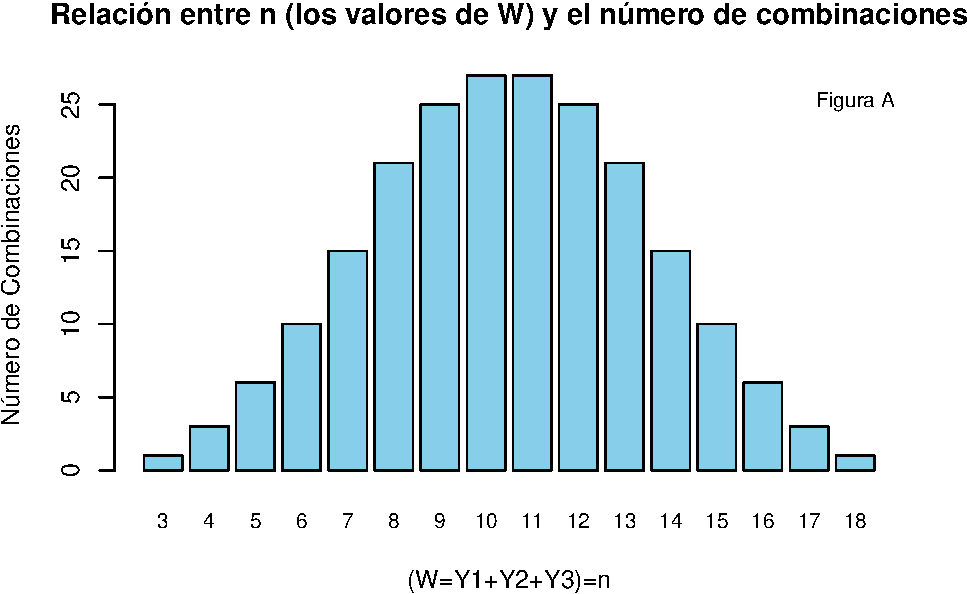
\includegraphics{inferencia_files/figure-latex/Figura (A)-1.pdf}

La probabilidad $\displaystyle P(\bar{Y}=\frac{n}{3})$ está determinada por la suma de las combinaciones posibles determinadas en R-software para que un $n$ tenga como resultado con $n \in \{3, \cdots, 18 \}$, lo cuál describe que es simétrica y la mayor concentración de los datos está alrededor de la media de $W$ y tiene forma de campana, por lo cuál es una distribución normal con las variables aleatorias. $Y_{1},Y_{2},Y_{3}$. 

\hypertarget{implementaciuxf3n-en-r-mediante-simulaciuxf3n}{%
\section{4. Implementación en R mediante
simulación}\label{implementaciuxf3n-en-r-mediante-simulaciuxf3n}}

En el siguiente espacio de código en R-Software se toma la muestra de las caras del dado (que es la población a estudiar) y con la función sample, se toman 3 valores arbitrarios de la muestra.

\newpage 

\begin{Shaded}
\begin{Highlighting}[]
\NormalTok{muestra }\OtherTok{\textless{}{-}} \FunctionTok{c}\NormalTok{(}\DecValTok{1}\NormalTok{,}\DecValTok{2}\NormalTok{,}\DecValTok{3}\NormalTok{,}\DecValTok{4}\NormalTok{,}\DecValTok{5}\NormalTok{,}\DecValTok{6}\NormalTok{)}
\NormalTok{tres\_valores\_arb }\OtherTok{\textless{}{-}} \FunctionTok{sample}\NormalTok{(muestra, }\DecValTok{3}\NormalTok{, }\AttributeTok{replace =} \ConstantTok{FALSE}\NormalTok{)}
\end{Highlighting}
\end{Shaded}

Ahora, tomamos un espacio muestral de 100 repeticiones del experimento y calculamos su media definida de la forma:

$$\bar{Y}=\frac{Y_{1}+Y_{2}+Y_{3}}{3} \hspace{1.5cm} (1)$$
En el siguiente código, realizamos una matriz de 4000 filas con 5 columnas y mostramos en el documento solo las primeras 6 filas donde las columnas $Y_{1}, Y_{2}, Y_{3}$ son las variables aleatorias, $W$ que es la suma $W=Y_{1}+Y_{2}+Y_{3}$ y la columna $Media$ es el cálculo de la media  definida con la ecuación (3.1) en cada una de las filas. 

\begin{Shaded}
\begin{Highlighting}[]
\FunctionTok{library}\NormalTok{(dplyr)}
\end{Highlighting}
\end{Shaded}

\begin{verbatim}
## 
## Attaching package: 'dplyr'
\end{verbatim}

\begin{verbatim}
## The following objects are masked from 'package:stats':
## 
##     filter, lag
\end{verbatim}

\begin{verbatim}
## The following objects are masked from 'package:base':
## 
##     intersect, setdiff, setequal, union
\end{verbatim}

\begin{Shaded}
\begin{Highlighting}[]
\CommentTok{\# Crear un vector de nombres para las columnas}
\NormalTok{nombres\_columnas }\OtherTok{\textless{}{-}} \FunctionTok{c}\NormalTok{(}\StringTok{"Y1"}\NormalTok{, }\StringTok{"Y2"}\NormalTok{, }\StringTok{"Y3"}\NormalTok{, }\StringTok{"W"}\NormalTok{, }\StringTok{"Media"}\NormalTok{)}

\CommentTok{\# Crear el dataframe vacío con los nombres de columnas adecuados}
\NormalTok{espacio\_muestral }\OtherTok{\textless{}{-}} \FunctionTok{data.frame}\NormalTok{(}\FunctionTok{matrix}\NormalTok{(}\FunctionTok{numeric}\NormalTok{(}\DecValTok{0}\NormalTok{), }\AttributeTok{nrow =} \DecValTok{0}\NormalTok{, }\AttributeTok{ncol =} \FunctionTok{length}\NormalTok{(nombres\_columnas)))}
\FunctionTok{names}\NormalTok{(espacio\_muestral) }\OtherTok{\textless{}{-}}\NormalTok{ nombres\_columnas}

\CommentTok{\# Generar los datos y agregarlos al dataframe}
\ControlFlowTok{for}\NormalTok{ (i }\ControlFlowTok{in} \DecValTok{1}\SpecialCharTok{:}\DecValTok{4000}\NormalTok{) \{}
\NormalTok{  tres\_valores\_arb }\OtherTok{\textless{}{-}} \FunctionTok{sample}\NormalTok{(muestra, }\DecValTok{3}\NormalTok{, }\AttributeTok{replace =} \ConstantTok{FALSE}\NormalTok{)}
\NormalTok{  w }\OtherTok{\textless{}{-}} \FunctionTok{sum}\NormalTok{(tres\_valores\_arb)  }\CommentTok{\# Calculamos W = Y1 + Y2 + Y3}
\NormalTok{  media\_definida }\OtherTok{\textless{}{-}} \FunctionTok{mean}\NormalTok{(tres\_valores\_arb)}
\NormalTok{  espacio\_muestral }\OtherTok{\textless{}{-}} \FunctionTok{rbind}\NormalTok{(espacio\_muestral, }\FunctionTok{c}\NormalTok{(tres\_valores\_arb, w, media\_definida))}
\NormalTok{\}}

\CommentTok{\# Renombrar las columnas del dataframe}
\NormalTok{espacio\_muestral }\OtherTok{\textless{}{-}}\NormalTok{ espacio\_muestral }\SpecialCharTok{\%\textgreater{}\%}
  \FunctionTok{setNames}\NormalTok{(nombres\_columnas)}
\FunctionTok{head}\NormalTok{(espacio\_muestral)}
\end{Highlighting}
\end{Shaded}

\begin{verbatim}
##   Y1 Y2 Y3  W    Media
## 1  5  1  4 10 3.333333
## 2  5  6  3 14 4.666667
## 3  5  6  1 12 4.000000
## 4  4  3  2  9 3.000000
## 5  4  5  2 11 3.666667
## 6  4  2  6 12 4.000000
\end{verbatim}

Ahora, por R-software, realizamos el histograma de los 4000 datos donde relacionaremos la frecuencia de los valores repetivos en $W = Y_{1}+Y_{2}+Y_{3}$ con los posibles valores que están en el cojunto $\{1, \cdots ,18\}$ y observamos la $\mu_{\bar{Y}}$ que es la media de las medias.

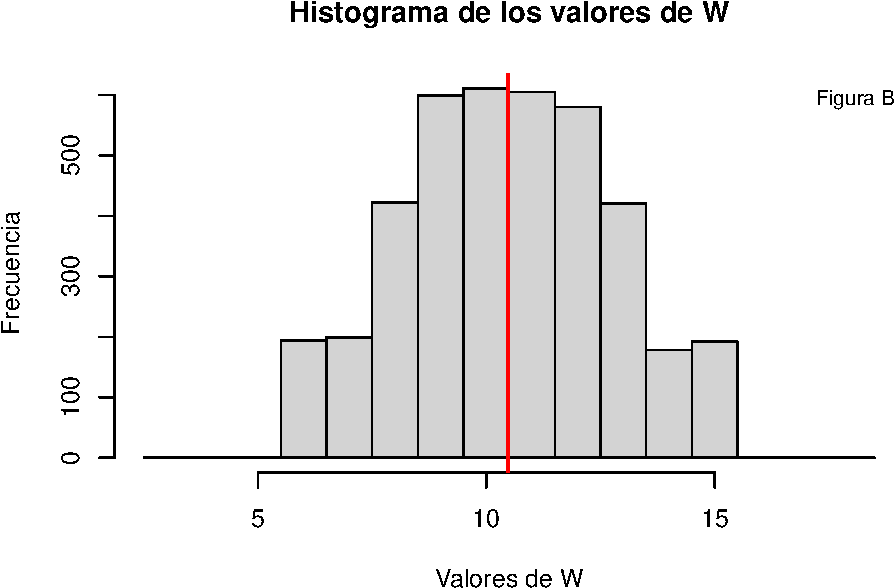
\includegraphics{inferencia_files/figure-latex/Figura (B)-1.pdf}

Lo que coincide el estudio teórico de la \textbf{Figura A} a la simulación de la  \textbf{Figura B} con valores de las variables aleatorias $Y_{1},Y_{2},Y_{3}$

\hypertarget{conclusiones}{%
\section{5. Conclusiones}\label{conclusiones}}

Al ser un dado justo (que no está cargado), lanzado 3 veces tal que 

$$\bar{Y} = \frac{W}{3} \text{  con  } W = Y_{1}+Y_{2}+Y_{3}$$

se logró responder las siguientes preguntas:

\begin{itemize}
  
  \item ¿Cuáles son la media $\mu_{\bar{Y}}$ y la desviación estándar $\sigma_{\bar{Y}}$ , de $\bar{Y}$?
  
  Con valores $Y_{1}=1,Y_{2}=2, Y_{3}=3$ el valor de la media es $\mu_{\bar{Y}} = 2$ y su desviación estándar $\sigma_{\bar{Y}} \approx .986013 $. La desviación es una medida de dispersión que nos indica cuánto varían estos valores promedio alrededor de la media, lo cuál es baja su variación.

  \item ¿Cómo podemos determinar la
distribución muestral de $\bar{Y}$ ?

Como la probabilidad $\displaystyle P(W=n)$ está determinada por la suma de las combinaciones posibles determinadas en R-software para que un $n$ tenga como resultado con $n \in \{3, \cdots, 18 \}$, lo que describe que es simétrica y la mayor concentración de los datos está alrededor de la media de $W$ ya que tiene una forma de campana, por lo cuál es una distribución normal con las variables aleatorias. $Y_{1},Y_{2},Y_{3}$. 

  \item Además, se simuló con valores aleatorios el lanzamiento de un dado, con R-Software comparando la frecuencia de $W$ con los valores esperados del conjunto $\{3,\cdots,18\}$ que fue el estudio teórico de las probabilidades que saliera un elemento del conjunto. Ambas figuras (A y B) coinciden dada la comparación.
\end{itemize}

\hypertarget{referencias}{%
\section{6. Referencias}\label{referencias}}

\begin{itemize}

  \item \textbf{Wackerly, Dennis D., William Mendenhall III, y Richard L. Scheaffer. Inferencia Estadística con aplicaciones. Séptima edición. Cengage Learning.}
  
  \item \textbf{Walpole, Ronald E., Raymond H. Myers, Sharon L. Myers, y Keying Ye. 2006. Probability and Statistics for Engineers and Scientists. 8ª edición. Prentice Hall.}

\end{itemize}

\end{document}
